% GENERATED by scripts/paper_figures.py from results/ -- do not edit
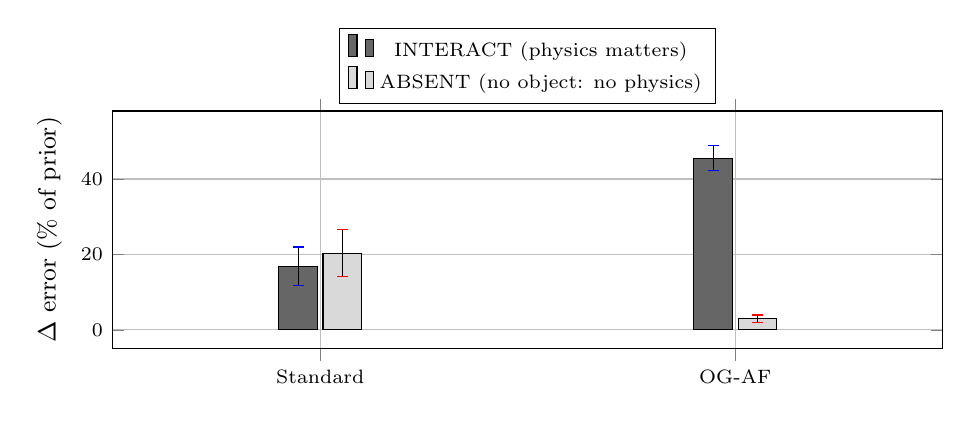
\begin{tikzpicture}\begin{axis}[width=\linewidth, height=4.6cm, ybar, bar width=14pt,
  symbolic x coords={Standard,OG-AF}, xtick=data, enlarge x limits=0.5, ymin=-5, ymax=58,
  ylabel={$\Delta$ error (\% of prior)}, grid=major,
  legend columns=1,
  legend style={font=\scriptsize, at={(0.5,1.03)}, anchor=south},
  tick label style={font=\scriptsize}, label style={font=\small}]
\addplot+[fill=black!60, draw=black, error bars/.cd, y dir=both, y explicit] coordinates {(Standard,16.898) +- (0,5.051) (OG-AF,45.488) +- (0,3.273)};\addlegendentry{INTERACT (physics matters)}
\addplot+[fill=black!15, draw=black, error bars/.cd, y dir=both, y explicit] coordinates {(Standard,20.277) +- (0,6.216) (OG-AF,2.924) +- (0,1.009)};\addlegendentry{ABSENT (no object: no physics)}
\end{axis}\end{tikzpicture}
